\documentclass[12pt,a4paper]{standalone}
\usepackage{amssymb}
\usepackage{amsmath}
\usepackage{bm}
\usepackage{tikz}
\usetikzlibrary{arrows.meta}
\usetikzlibrary{arrows}
\usepackage{pstricks}
\usetikzlibrary{patterns}
\usetikzlibrary{fadings}
\usetikzlibrary{shapes.geometric}







\begin{document}
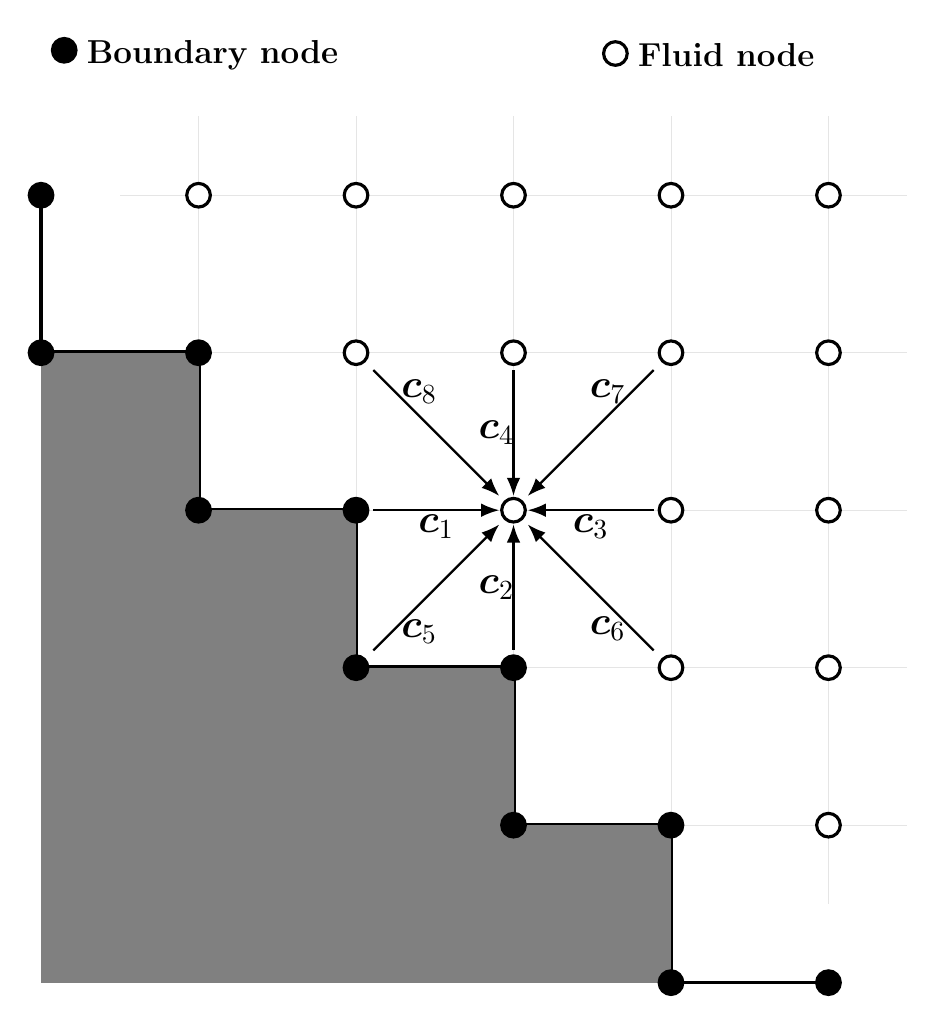
\begin{tikzpicture}[line width=0.4mm,>=Latex]
%\draw[dashed,thick,line width=0.6mm] (4,2) -- (7.7,7.4);

%\fill[black!10] (6,4) rectangle (8,6);
%\fill[black!10] (8,4) rectangle (10,6);
%\fill[black!10] (6,2) rectangle (8,6);
%\fill[black!10] (8,2) rectangle (10,4);



\draw[gray!20,solid,thick,line width=0.1mm] (3,0) -- (13,0);
\draw[gray!20,solid,thick,line width=0.1mm] (3,2) -- (13,2);
\draw[gray!20,solid,thick,line width=0.1mm] (3,4) -- (13,4);
\draw[gray!20,solid,thick,line width=0.1mm] (3,6) -- (13,6);
\draw[gray!20,solid,thick,line width=0.1mm] (3,8) -- (13,8);

%\draw[gray!20,solid,thick,line width=0.1mm] (2,-1) -- (2,9);
\draw[gray!20,solid,thick,line width=0.1mm] (4,-1) -- (4,9);
\draw[gray!20,solid,thick,line width=0.1mm] (6,-1) -- (6,9);
\draw[gray!20,solid,thick,line width=0.1mm] (8,-1) -- (8,9);
\draw[gray!20,solid,thick,line width=0.1mm] (10,-1) -- (10,9);
\draw[gray!20,solid,thick,line width=0.1mm] (12,-1) -- (12,9);

%\draw[thick,line width=1mm] (10.2,-0.6) arc[start angle=15, end angle=78, radius=9.66];
%\draw[pattern=north west lines, pattern color=gray!80] (6,4) rectangle (8,6);
%\draw[pattern=north east lines, pattern color=gray] (6,6) rectangle (8,8);

\draw[solid,thick,line width=0.4mm] (2,8) -- (2,6);
\draw[solid,thick,line width=0.6mm] (2,6) -- (4,6);
\draw[solid,thick,line width=0.6mm] (4,6) -- (4,4);
\draw[solid,thick,line width=0.6mm] (4,4) -- (6,4);
\draw[solid,thick,line width=0.6mm] (6,4) -- (6,2);
\draw[solid,thick,line width=0.6mm] (6,2) -- (8,2);
\draw[solid,thick,line width=0.6mm] (8,2) -- (8,0);
\draw[solid,thick,line width=0.6mm] (8,0) -- (10,0);
\draw[solid,thick,line width=0.6mm] (10,0) -- (10,-2);
\draw[solid,thick,line width=0.4mm] (10,-2) -- (12,-2);


\fill[black!50] (2,4) rectangle (4,6);
%\fill[pattern=north east lines, pattern color=black!60]
%(2,6) -- (2,4) -- (4,4) --(4,6) -- cycle;

\fill[black!50] (4,2) rectangle (6,4);
%\fill[pattern=north east lines, pattern color=black!60]
%(4,4) -- (4,2) -- (6,2) --(6,4) -- cycle;

\fill[black!50] (6,0) rectangle (8,2);
%\fill[pattern=north east lines, pattern color=black!60]
%(6,2) -- (6,0) -- (8,0) --(8,2) -- cycle;

\fill[black!50] (8,-2) rectangle (10,0);
%\fill[pattern=north east lines, pattern color=black!60]
%(8,0) -- (8,-2) -- (10,-2) --(10,0) -- cycle;


\fill[black!50] (4,0) rectangle (6,2);




\fill[black!50] (2,2) rectangle (4,4);
\fill[black!50] (2,0) rectangle (4,2);

\fill[black!50] (2,-2) rectangle (4,0);
\fill[black!50] (4,-2) rectangle (6,0);
\fill[black!50] (6,-2) rectangle (8,0);


%\fill[pattern=north east lines, pattern color=black!50]
%(2,8) -- (2,6) -- (4,6) --(4,8) -- cycle;
%
%\fill[pattern=north east lines, pattern color=black!50]
%(4,4) -- (6,4) -- (6,6) --(4,6) -- cycle;
%
%\fill[pattern=north east lines, pattern color=black!50]
%(6,2) -- (8,2) -- (8,4) --(6,4) -- cycle;
%
%\fill[pattern=north east lines, pattern color=black!50]
%(8,0) -- (10,0) -- (10,2) --(8,2) -- cycle;
%
%\fill[pattern=north east lines, pattern color=black!50]
%(10,-2) -- (12,-2) -- (12,0) --(10,0) -- cycle;



%top first row
\draw[black,fill=black] (2,8)node[]{} circle(0.15cm);
\draw[black,fill=white] (4,8)node[]{} circle(0.15cm);
\draw[black,fill=white] (6,8)node[]{} circle(0.15cm);
\draw[black,fill=white] (8,8)node[]{} circle(0.15cm);
\draw[black,fill=white] (10,8)node[]{} circle(0.15cm);
\draw[black,fill=white] (12,8)node[]{} circle(0.15cm);

%top second row

\draw[black,fill=black] (2,6)node[]{} circle(0.15cm);
\draw[black,fill=black] (4,6)node[]{} circle(0.15cm);
\draw[black,fill=white] (6,6)node[]{} circle(0.15cm);
\draw[black,fill=white] (8,6)node[]{} circle(0.15cm);
\draw[black,fill=white] (10,6)node[]{} circle(0.15cm);
\draw[black,fill=white] (12,6)node[]{} circle(0.15cm);



% arrow parameters
\def\rstart{0.18}   % distance from center
\def\rlen{1.6}      % arrow length


\draw[black, thick, {Latex}-]
(8,4) ++(\rstart,0) -- ++(\rlen,0)
node[midway,below, yshift=2pt,font=\fontsize{14pt}{12pt}\selectfont] {$\bm{c}_3$};

% up (2)
\draw[black, thick, {Latex}-]
(8,4) ++(0,\rstart) -- ++(0,\rlen)
node[midway, left, xshift=4pt,font=\fontsize{14pt}{12pt}\selectfont] {$\bm{c}_4$};

% left (3)
\draw[black, thick, {Latex}-]
(8,4) ++(-\rstart,0) -- ++(-\rlen,0)
node[midway, below, yshift=2pt,font=\fontsize{14pt}{12pt}\selectfont] {$\bm{c}_1$};

% down (4)
\draw[black, thick, {Latex}-]
(8,4) ++(0,-\rstart) -- ++(0,-\rlen)
node[midway, left, xshift=4pt,font=\fontsize{14pt}{12pt}\selectfont] {$\bm{c}_2$};

% diagonals
\draw[black, thick, {Latex}-]
(8,4) ++(\rstart,\rstart) -- ++(\rlen,\rlen)
node[midway, above right,xshift=-4pt, yshift=7pt,font=\fontsize{14pt}{12pt}\selectfont] {$\bm{c}_7$};

\draw[black, thick, {Latex}-]
(8,4) ++(\rstart,-\rstart) -- ++(\rlen,-\rlen)
node[midway, below right,xshift=-4pt, yshift=-7pt,font=\fontsize{14pt}{12pt}\selectfont] {$\bm{c}_6$};

\draw[black, thick, {Latex}-]
(8,4) ++(-\rstart,\rstart) -- ++(-\rlen,\rlen)
node[midway, above left,xshift=4pt, yshift=7pt,font=\fontsize{14pt}{12pt}\selectfont] {$\bm{c}_8$};

\draw[black, thick, {Latex}-]
(8,4) ++(-\rstart,-\rstart) -- ++(-\rlen,-\rlen)
node[midway, below left,xshift=4pt, yshift=-8pt,font=\fontsize{14pt}{12pt}\selectfont] {$\bm{c}_5$};



\draw[black,fill=black] (4,4)node[]{} circle(0.15cm);
\draw[black,fill=black] (6,4)node[]{} circle(0.15cm);
\draw[black,fill=white] (8,4)node[]{} circle(0.15cm);
\draw[black,fill=white] (10,4)node[]{} circle(0.15cm);
\draw[black,fill=white] (12,4)node[]{} circle(0.15cm);

%top fourth row
%\node [draw, gray, fill=white,diamond, aspect=1,scale=0.7] at (2,2) {};
%\node [draw, gray, fill=white,diamond, aspect=1,scale=0.7] at (4,2) {};
\draw[black,fill=black] (6,2)node[]{} circle(0.15cm);
\draw[black,fill=black] (8,2)node[]{} circle(0.15cm);
\draw[black,fill=white] (10,2)node[]{} circle(0.15cm);
\draw[black,fill=white] (12,2)node[]{} circle(0.15cm);

%top fifth row
%\node [draw, gray, fill=white,diamond, aspect=1,scale=0.7] at (2,0) {};
%\node [draw, gray, fill=white,diamond, aspect=1,scale=0.7] at (4,0) {};
%\node [draw, gray, fill=white,diamond, aspect=1,scale=0.7] at (6,0) {};
\draw[black,fill=black] (8,0)node[]{} circle(0.15cm);
\draw[black,fill=black] (10,0)node[]{} circle(0.15cm);
\draw[black,fill=white] (12,0)node[]{} circle(0.15cm);

\draw[black,fill=black] (10,-2)node[]{} circle(0.15cm);
\draw[black,fill=black] (12,-2)node[]{} circle(0.15cm);


\tikzset{solid_node/.style={draw=black, fill=black, line width=0.4mm, circle, minimum size=0.3cm, inner sep=0pt}}
\tikzset{fluid_node/.style={draw=black, fill=white,line width=0.4mm, circle, minimum size=0.3cm, inner sep=0pt}}

\draw (2,9.8) node[anchor=west] { \tikz{\node[solid_node] {};} {\large\textbf{Boundary node}} };
\draw (9,9.8) node[anchor=west] { \tikz{\node[fluid_node] {};} {\large\textbf{Fluid node}} };
\end{tikzpicture}



\end{document}



